\documentclass[12pt]{paper}
\usepackage{amsmath}
\usepackage{amssymb}
\usepackage{graphicx}
\usepackage{hyperref}
\usepackage{color}
\begin{document}
\title{Signaling and Chromatin Structure}
\maketitle

In this document I will try to summarize all the necessary information related to the construction of a model, linking signaling at the nuclear membrane, and its affect on the micro-structure of the chromatin.

\subsection{Assumptions}
\begin{enumerate}
\item We assume the chromosome is represented by bead-strings model. 
\item The beads are the histone proteins on which the DNA is coiled.
\item Beads have attraction or repulsion forces between them, governed by methylation/phosphorylation state.
\item Methylation or phosphorylation is governed by the activation or repression of a certain process, which requires the access to a particular region along the chromatin. 
\item The activation and repression are those of a general process, which activatesa cascade of events that finally requires access to a physical location of the DNA. 
\item Many activation/repression can occur simultaneously on overlapping regions of the chromatin. 
\item The effect of the activation is translated into contracting/repulsion force between histones.
\item The force has a range of activation in a finite support with weak influence on the boundaries in comparison to the center of the region.
\item The contraction/repulsion is caused by active protein, scanning or working on the strand of DNA.

\end{enumerate}

\begin{figure}[h!]
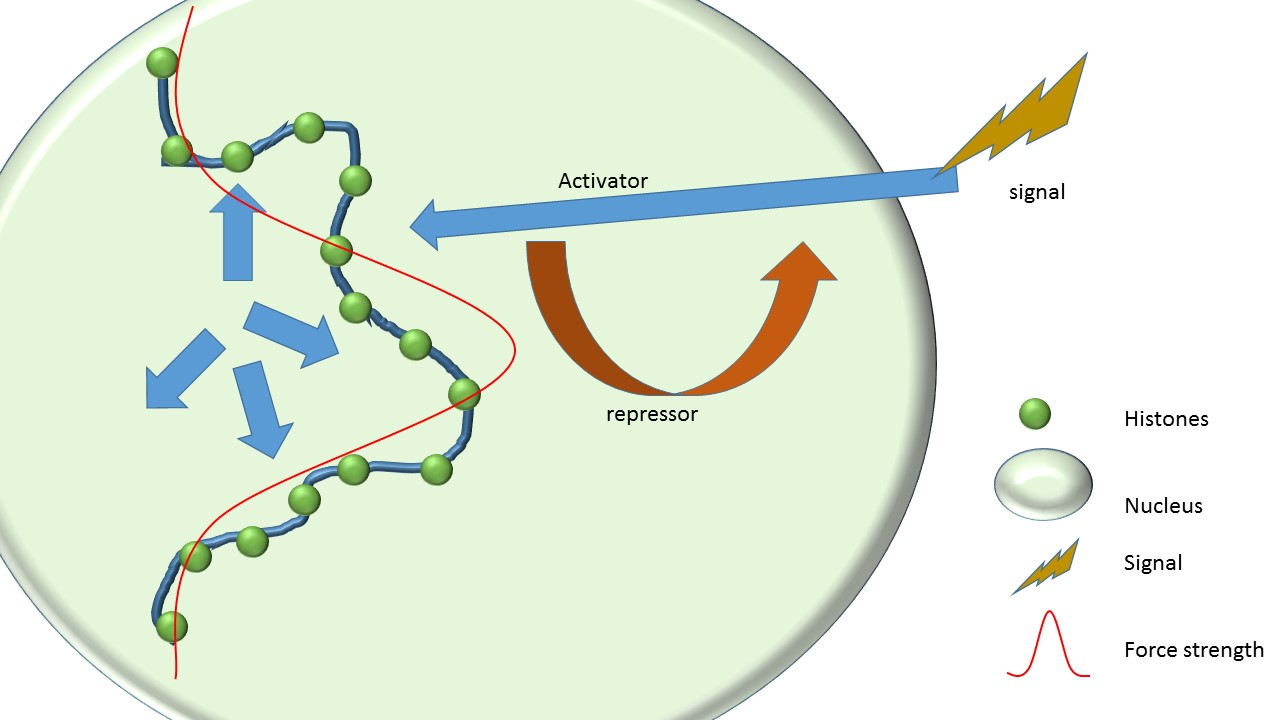
\includegraphics[scale=0.4]{modelSketch}
\end{figure}

The main idea is to simulate the shape of the chromatin as a function of the input signal (activator) and repression of that signal. We want to show that creation of discrete regions have to do with functionality and not just compaction. The simulation of euchromatin and heterochromatin should be possible by this model. Then, gene activation, including stochastic gene activation, can be shown to be dependent on the signals received from the cell membrane and thier repression. The steady-state structure of the chromatin will depend on the pattern of signaling and their spatial affect. 

Furthermore, we want to show that this model exerts optimal search times of transcription factor with minimal amount of resources. In the resulting architecture, phenomena like the TADs can be shown to be a particular pattern of the model. We then hypothesis that active regions and inactive/dense chromatin region (type A and B in some literature) might show a similar encounter probability pattern in the HiC experiment.


\subsection{Activator repressor model}
We model a general process with feedback as the simplest model available, namely a Lotka voltera model of prey predator 
\begin{eqnarray}
\frac{dA(t)}{dt} &=& \alpha A(t)- \beta A(t)R(t)\\
\frac{dR(t)}{dt} &=& \gamma A(t)R(t)-\delta R(t)
\end{eqnarray}
with $A(t)$ the activator concentration/strength at time $t$, $R(t)$ the repressor concentration/ strength at time $t$, $\alpha$ the activator birth rate, $\beta$ activator death rate as a result of interaction with the repressor, $\gamma$ repressor birth rate as a result of interaction with the activator (maybe recruiting rate?), and $\delta$ the repressor death rate.
To take into account only one term in the model, we calculate the difference between the activation and repression. 

\subsection{Force influence}
The influence of the force on the chain should be modeled spatially with (perhaps) a Gaussian function. This influence will be embodied in the term for the chain's potential as the external field.  The force exerted on the chain should push beads (histons) apart when applied. This assumption needs to be supported by the simple situation in which a Rouse chain, encored in both ends is felt a force on the middle beads in an outward manner. 

\begin{figure}[h~]
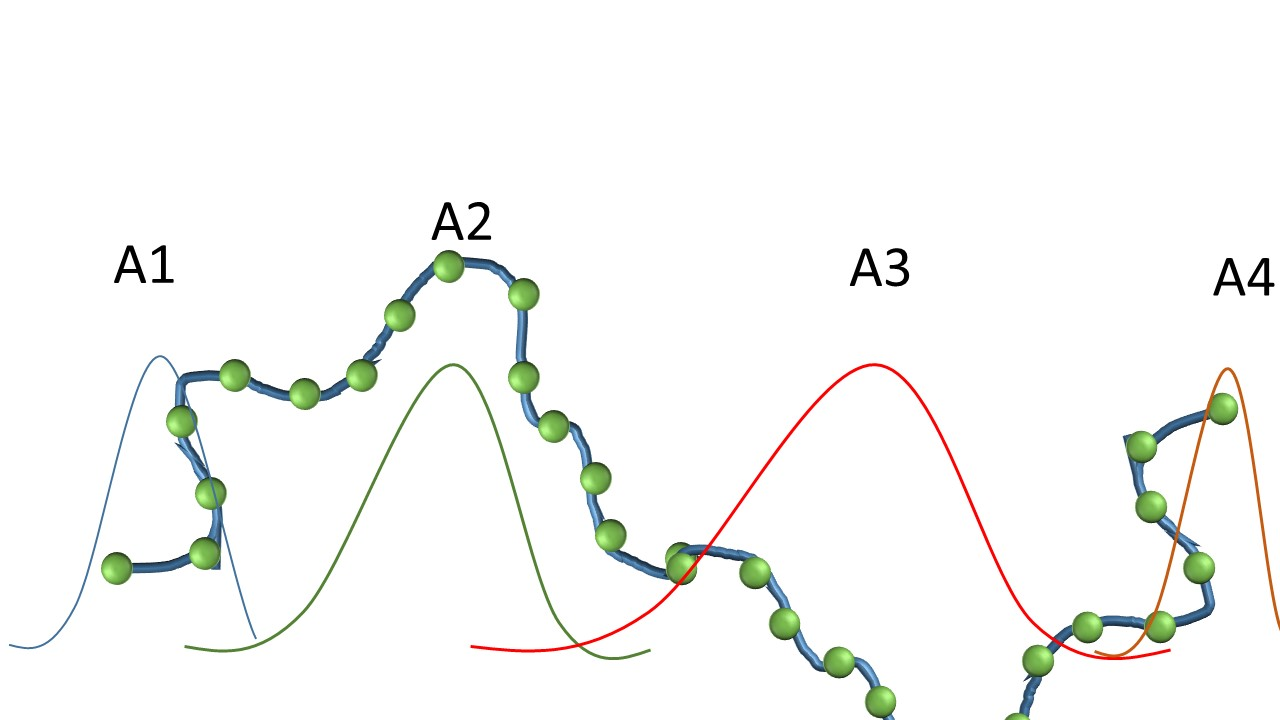
\includegraphics[scale=0.4]{forceInfluenceOnChain}
\caption{many activation/repression signals can operate simultaneously on the chromatin $A_1,A_2,...A_N$, wach one exerts force on a specific part of the chromatin, with larger influence in the middl of the region than at its boundaries. The considerations for such force comes from the assumptions that proteins are working on this particular DNA segment and they 'push' the segments apart by detaching the histone connectivity or by exerting physical force. In the absence of external force (in the repression stage) the histone tend to grooup together due to the contracting force}
\label{foce influence on the chromatin dynamics}
\end{figure}

The equilibrium distribution is changed by a factor of 
\begin{equation}
\exp\left(\frac{1}{K_BT}\int_{0}^NU_e(R_n(t))dn\right)
\end{equation}

where $U_e(R_n(t))$ represents the external field at time $t$ on all beads $R_n=\{r_1,r_2,...,r_n\}$
\end{document}